% Schematic of direct (classical) Thomson scattering.
% An incident low-frequency electromagnetic wave / photon of frequency omega_0
% hits a stationary free electron, driving it into oscillation; the electron
% re-radiates a scattered photon at angle theta with the same frequency (omega_1 = omega_0).
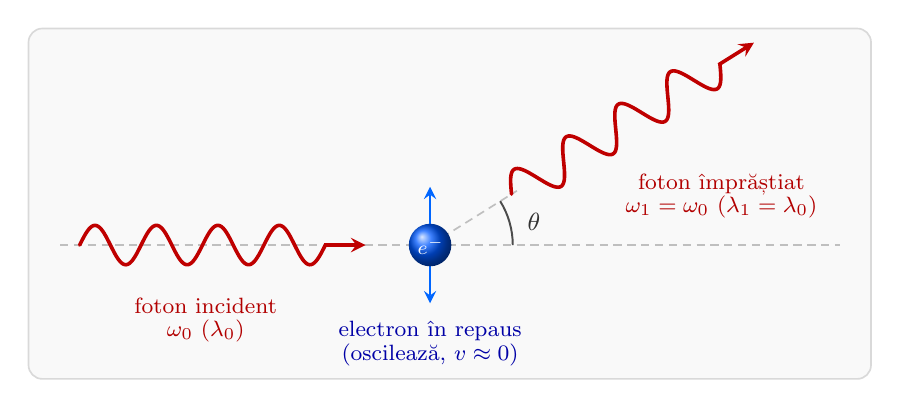
\begin{tikzpicture}[>=stealth, font=\footnotesize]
  % Outer soft card matching inverse_thomson_scattering.tex style
  \filldraw[fill=gray!5, draw=gray!30, rounded corners=5pt, line width=0.6pt]
    (-0.20, -1.70) rectangle (10.50, 2.75);

  % Optical axis and scattered propagation ray (dashed, behind electron)
  \draw[gray!50, densely dashed, line width=0.6pt] (0.20, 0.00) -- (10.10, 0.00);
  \draw[gray!50, densely dashed, line width=0.6pt] (4.90, 0.00) -- ++(32:1.30);

  % Incident photon (red sine wave moving right along +x, 4 cycles of lambda = 0.78)
  \draw[red!75!black, line width=1.3pt, line cap=round,
    domain=0.45:3.57, samples=160, variable=\x, smooth]
    plot (\x, {0.25*sin(deg(2*pi*(\x - 0.45)/0.78))});
  \draw[->, red!75!black, line width=1.3pt] (3.55, 0.00) -- (4.08, 0.00);

  \node[red!70!black, align=center] at (2.05, -0.95)
    {foton incident\\[-1pt]$\omega_0$ ($\lambda_0$)};

  % Vertical oscillation indicator on the electron
  \draw[<->, blue!60!cyan, line width=0.95pt] (4.90, -0.74) -- (4.90, 0.74);

  % Stationary (oscillating) electron at (4.90, 0)
  \shade[ball color=blue!65!cyan] (4.90, 0.00) circle (0.27);
  \node[white, font=\scriptsize\bfseries] at (4.91, -0.01) {$e^-$};

  \node[blue!65!black, align=center] at (4.90, -1.25)
    {electron în repaus\\[-1pt](oscilează, $v \approx 0$)};

  % Clean angle arc (theta = 32 deg)
  \draw[black!70, line width=0.7pt] (5.95, 0.00) arc[start angle=0, end angle=32, radius=1.05];
  \node[black!80, font=\small] at (6.22, 0.30) {$\theta$};

  % Scattered photon (same color and SAME wavelength = 0.78, moving at 32 deg)
  \begin{scope}[shift={(4.90, 0.00)}, rotate=32]
    \draw[red!75!black, line width=1.3pt, line cap=round,
      domain=1.22:4.34, samples=160, variable=\x, smooth]
      plot (\x, {0.25*sin(deg(2*pi*(\x - 1.22)/0.78))});
    \draw[->, red!75!black, line width=1.3pt] (4.32, 0.00) -- (4.85, 0.00);
  \end{scope}

  \node[red!70!black, align=center] at (8.60, 0.62)
    {foton împrăștiat\\[-1pt]$\omega_1 = \omega_0$ ($\lambda_1 = \lambda_0$)};
\end{tikzpicture}
